% /home/nlct/programming/java/jpgfdraw/trunk/doc/image-src/editText.jdr
% Created by FlowframTk version 0.6
% 24-May-2014 17:06:46
\iffalse
% This image may require the following commands in the preamble:
\usepackage{ifpdf}
\makeatletter
\ifpdf
 \input{pdf-trans}
 \newcommand*{\jdroutline}[3]{%
   \setbox\@tempboxa\hbox{#3}%
   \boxgs{#1}{}\copy\@tempboxa
 }
\else
 \usepackage{pst-char}
 \newcommand*{\jdroutline}[3]{%
   \begin{pspicture}(0,0)
   \pscharpath[#2]{#3}
   \end{pspicture}
 }
\fi
\makeatother
\usepackage{pgf}
\usepgflibrary{decorations.text}
% The normal size font is assumed to be 10pt
% End of preamble information
\fi
\begin{pgfpicture}{62.0bp}{465.378642bp}{454.0bp}{760.503642bp}
\begin{pgfscope}
\pgftransformcm{1.0}{0.0}{0.0}{1.0}{\pgfpoint{62.0bp}{703.889764bp}}
\pgflowlevelsynccm
\pgfputat{\pgfpoint{0pt}{0pt}}{\pgftext[top,left]{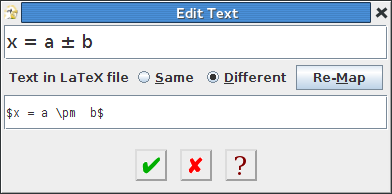
\includegraphics[width=392.0bp,height=194.0bp]{editTextsnapshot}}}
\end{pgfscope}
\begin{pgfscope}
\pgftransformcm{1.0}{-0.0}{0.0}{1.0}{\pgfpoint{225.474348bp}{737.381767bp}}
\pgftext[center,base]{\rmfamily\mdseries\upshape\normalsize\color[rgb]{0.0,0.0,0.0}in text area}
\end{pgfscope}
\begin{pgfscope}
\pgftransformcm{1.0}{-0.0}{0.0}{1.0}{\pgfpoint{225.474348bp}{753.581767bp}}
\pgftext[center,base]{\rmfamily\mdseries\upshape\normalsize\color[rgb]{0.0,0.0,0.0}Text to appear}
\end{pgfscope}
\begin{pgfscope}
\pgftransformcm{1.0}{-0.0}{0.0}{1.0}{\pgfpoint{115.474348bp}{480.381767bp}}
\pgftext[center,base]{\rmfamily\mdseries\upshape\normalsize\color[rgb]{0.0,0.0,0.0}Text to appear}
\end{pgfscope}
\begin{pgfscope}
\pgftransformcm{1.0}{-0.0}{0.0}{1.0}{\pgfpoint{115.474348bp}{465.581767bp}}
\pgftext[center,base]{\rmfamily\mdseries\upshape\normalsize\color[rgb]{0.0,0.0,0.0}in LaTeX file}
\end{pgfscope}
\begin{pgfscope}
\pgfsetlinewidth{1.0bp}
\pgfsetrectcap
\pgfsetmiterjoin
\pgfsetmiterlimit{10.0}
\pgfpathmoveto{\pgfpoint{115.474349bp}{579.689764bp}}
\pgfpathlineto{\pgfpoint{115.474349bp}{493.289764bp}}
\definecolor{strokepaint}{rgb}{0.0,0.0,0.0}\pgfsetstrokecolor{strokepaint}
\pgfusepath{stroke}
\end{pgfscope}
% marker type 7
{\begin{pgfscope}
\definecolor{fillpaint}{rgb}{0.0,0.0,0.0}\pgfsetfillcolor{fillpaint}
\pgfpathqmoveto{115.47435bp}{581.689752bp}
\pgfpathqlineto{119.47435bp}{573.689752bp}
\pgfpathqlineto{115.47435bp}{576.689752bp}
\pgfpathqlineto{111.47435bp}{573.689752bp}
\pgfclosepath
\pgfusepathqfill
\end{pgfscope}}
\begin{pgfscope}
\pgfsetlinewidth{1.0bp}
\pgfsetrectcap
\pgfsetmiterjoin
\pgfsetmiterlimit{10.0}
\pgfpathmoveto{\pgfpoint{164.799988bp}{668.053765bp}}
\pgfpathlineto{\pgfpoint{225.6bp}{729.053765bp}}
\definecolor{strokepaint}{rgb}{0.0,0.0,0.0}\pgfsetstrokecolor{strokepaint}
\pgfusepath{stroke}
\end{pgfscope}
% marker type 7
{\begin{pgfscope}
\definecolor{fillpaint}{rgb}{0.0,0.0,0.0}\pgfsetfillcolor{fillpaint}
\pgfpathqmoveto{163.388092bp}{666.637231bp}
\pgfpathqlineto{166.202591bp}{675.127145bp}
\pgfpathqlineto{166.917816bp}{670.178567bp}
\pgfpathqlineto{171.868729bp}{669.479592bp}
\pgfclosepath
\pgfusepathqfill
\end{pgfscope}}
\end{pgfpicture}
